% !TEX TS-program = pdflatex
% !TEX encoding = UTF-8 Unicode

% This is a simple template for a LaTeX document using the "article" class.
% See "book", "report", "letter" for other types of document.

\documentclass[11pt]{article} % use larger type; default would be 10pt

\usepackage[utf8]{inputenc} % set input encoding (not needed with XeLaTeX)
\usepackage{tikz}
%%% Examples of Article customizations
% These packages are optional, depending whether you want the features they provide.
% See the LaTeX Companion or other references for full information.

%%% PAGE DIMENSIONS
\usepackage{geometry} % to change the page dimensions
\geometry{a4paper} % or letterpaper (US) or a5paper or....
% \geometry{margins=2in} % for example, change the margins to 2 inches all round
% \geometry{landscape} % set up the page for landscape
%   read geometry.pdf for detailed page layout information

\usepackage{graphicx} % support the \includegraphics command and options

% \usepackage[parfill]{parskip} % Activate to begin paragraphs with an empty line rather than an indent

%%% PACKAGES
\usepackage{booktabs} % for much better looking tables
\usepackage{array} % for better arrays (eg matrices) in maths
\usepackage{paralist} % very flexible & customisable lists (eg. enumerate/itemize, etc.)
\usepackage{verbatim} % adds environment for commenting out blocks of text & for better verbatim
\usepackage{subfig} % make it possible to include more than one captioned figure/table in a single float
% These packages are all incorporated in the memoir class to one degree or another...
\usepackage{url}
\usepackage{hyperref}

%%% HEADERS & FOOTERS
\usepackage{fancyhdr} % This should be set AFTER setting up the page geometry
\pagestyle{fancy} % options: empty , plain , fancy
\renewcommand{\headrulewidth}{0pt} % customise the layout...
\lhead{}\chead{}\rhead{}
\lfoot{}\cfoot{\thepage}\rfoot{}

%%% SECTION TITLE APPEARANCE
\usepackage{sectsty}
\allsectionsfont{\sffamily\mdseries\upshape} % (See the fntguide.pdf for font help)
% (This matches ConTeXt defaults)

%%% ToC (table of contents) APPEARANCE
\usepackage[nottoc,notlof,notlot]{tocbibind} % Put the bibliography in the ToC
\usepackage[titles,subfigure]{tocloft} % Alter the style of the Table of Contents
\renewcommand{\cftsecfont}{\rmfamily\mdseries\upshape}
\renewcommand{\cftsecpagefont}{\rmfamily\mdseries\upshape} % No bold!

%%% END Article customizations

%%% The "real" document content comes below...

\usepackage{amsfonts}
\usepackage{amsmath}
\usepackage{amsthm}

\theoremstyle{definition}
\newtheorem*{beispiel}{Beispiel}
\newtheorem{definition}{Definition}
\newtheorem*{bemerkung}{Bemerkung}
\newtheorem*{beweis}{Beweis}
\newtheorem*{ubung}{Übung}

\title{Übungsblatt 1}
\author{Florian}
%\date{} % Activate to display a given date or no date (if empty),
         % otherwise the current date is printed 

\begin{document}
\maketitle

\section*{Aufgabe 1}

\begin{enumerate}[a)] 

\item Die Auftretenswahrscheinlichkeiten $p(x)$ (wobei $\sum\limits_{x\in A} p(x) = 2.98$) werden normiert auf $1.0$.
\begin{eqnarray*}
E(A) &=& \sum\limits_{x \in A} p(x) \cdot \log_2 \frac{1}{p(x)} \\
&=& 10\cdot \frac {0.1}{2.98}\cdot \log_2\frac{2.98}{0.1}
+ \frac{0.13}{2.98}\cdot\log_2\frac{2.98}{0.13}
+ \frac{0.15}{2.98}\cdot\log_2\frac{2.98}{0.15}\\
&&+ \frac{0.20}{2.98}\cdot\log_2\frac{2.98}{0.20}
+ \frac{0.5}{2.98}\cdot\log_2\frac{2.98}{0.5}
+ \frac{0.4}{2.98}\cdot\log_2\frac{2.98}{0.4}
+ \frac{0.6}{2.98}\cdot\log_2\frac{2.98}{0.6} \\
&=& 3.60565808338531\dots
\end{eqnarray*}

\item Nur Blätter:\begin{center}
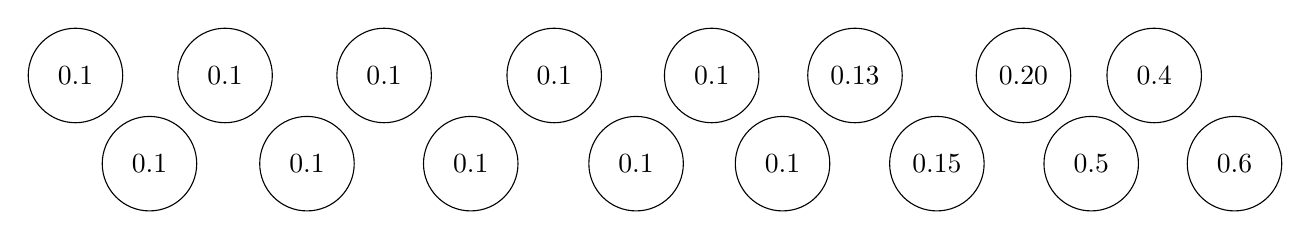
\begin{tikzpicture}[scale=0.2]
\tikzstyle{every node}+=[inner sep=0pt]
\draw [black] (3,-48.3) circle (3);
\draw (3,-48.3) node {$0.1$};
\draw [black] (7.7,-53.9) circle (3);
\draw (7.7,-53.9) node {$0.1$};
\draw [black] (12.5,-48.3) circle (3);
\draw (12.5,-48.3) node {$0.1$};
\draw [black] (52.5,-48.3) circle (3);
\draw (52.5,-48.3) node {$0.13$};
\draw [black] (63.2,-48.3) circle (3);
\draw (63.2,-48.3) node {$0.20$};
\draw [black] (43.4,-48.3) circle (3);
\draw (43.4,-48.3) node {$0.1$};
\draw [black] (57.7,-53.9) circle (3);
\draw (57.7,-53.9) node {$0.15$};
\draw [black] (33.4,-48.3) circle (3);
\draw (33.4,-48.3) node {$0.1$};
\draw [black] (28.1,-53.9) circle (3);
\draw (28.1,-53.9) node {$0.1$};
\draw [black] (22.6,-48.3) circle (3);
\draw (22.6,-48.3) node {$0.1$};
\draw [black] (17.7,-53.9) circle (3);
\draw (17.7,-53.9) node {$0.1$};
\draw [black] (47.9,-53.9) circle (3);
\draw (47.9,-53.9) node {$0.1$};
\draw [black] (38.6,-53.9) circle (3);
\draw (38.6,-53.9) node {$0.1$};
\draw [black] (67.5,-53.9) circle (3);
\draw (67.5,-53.9) node {$0.5$};
\draw [black] (71.5,-48.3) circle (3);
\draw (71.5,-48.3) node {$0.4$};
\draw [black] (76.6,-53.9) circle (3);
\draw (76.6,-53.9) node {$0.6$};
\end{tikzpicture}
\end{center}

Die 10 0.1-er zusammengefasst:
\begin{center}
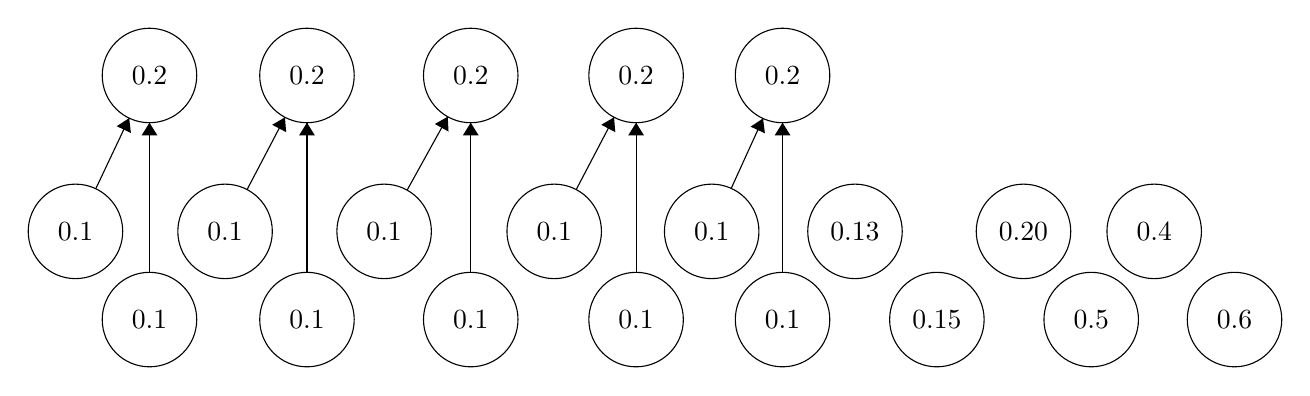
\begin{tikzpicture}[scale=0.2]
\tikzstyle{every node}+=[inner sep=0pt]
\draw [black] (3,-48.3) circle (3);
\draw (3,-48.3) node {$0.1$};
\draw [black] (7.7,-53.9) circle (3);
\draw (7.7,-53.9) node {$0.1$};
\draw [black] (12.5,-48.3) circle (3);
\draw (12.5,-48.3) node {$0.1$};
\draw [black] (52.5,-48.3) circle (3);
\draw (52.5,-48.3) node {$0.13$};
\draw [black] (63.2,-48.3) circle (3);
\draw (63.2,-48.3) node {$0.20$};
\draw [black] (43.4,-48.3) circle (3);
\draw (43.4,-48.3) node {$0.1$};
\draw [black] (57.7,-53.9) circle (3);
\draw (57.7,-53.9) node {$0.15$};
\draw [black] (33.4,-48.3) circle (3);
\draw (33.4,-48.3) node {$0.1$};
\draw [black] (28.1,-53.9) circle (3);
\draw (28.1,-53.9) node {$0.1$};
\draw [black] (22.6,-48.3) circle (3);
\draw (22.6,-48.3) node {$0.1$};
\draw [black] (17.7,-53.9) circle (3);
\draw (17.7,-53.9) node {$0.1$};
\draw [black] (47.9,-53.9) circle (3);
\draw (47.9,-53.9) node {$0.1$};
\draw [black] (38.6,-53.9) circle (3);
\draw (38.6,-53.9) node {$0.1$};
\draw [black] (67.5,-53.9) circle (3);
\draw (67.5,-53.9) node {$0.5$};
\draw [black] (71.5,-48.3) circle (3);
\draw (71.5,-48.3) node {$0.4$};
\draw [black] (76.6,-53.9) circle (3);
\draw (76.6,-53.9) node {$0.6$};
\draw [black] (7.7,-38.4) circle (3);
\draw (7.7,-38.4) node {$0.2$};
\draw [black] (17.7,-38.4) circle (3);
\draw (17.7,-38.4) node {$0.2$};
\draw [black] (28.1,-38.4) circle (3);
\draw (28.1,-38.4) node {$0.2$};
\draw [black] (38.6,-38.4) circle (3);
\draw (38.6,-38.4) node {$0.2$};
\draw [black] (47.9,-38.4) circle (3);
\draw (47.9,-38.4) node {$0.2$};
\draw [black] (4.29,-45.59) -- (6.41,-41.11);
\fill [black] (6.41,-41.11) -- (5.62,-41.62) -- (6.52,-42.05);
\draw [black] (7.7,-50.9) -- (7.7,-41.4);
\fill [black] (7.7,-41.4) -- (7.2,-42.2) -- (8.2,-42.2);
\draw [black] (13.9,-45.64) -- (16.3,-41.06);
\fill [black] (16.3,-41.06) -- (15.49,-41.53) -- (16.38,-42);
\draw [black] (17.7,-50.9) -- (17.7,-41.4);
\fill [black] (17.7,-41.4) -- (17.2,-42.2) -- (18.2,-42.2);
\draw [black] (24.06,-45.68) -- (26.64,-41.02);
\fill [black] (26.64,-41.02) -- (25.82,-41.48) -- (26.69,-41.96);
\draw [black] (28.1,-50.9) -- (28.1,-41.4);
\fill [black] (28.1,-41.4) -- (27.6,-42.2) -- (28.6,-42.2);
\draw [black] (34.8,-45.64) -- (37.2,-41.06);
\fill [black] (37.2,-41.06) -- (36.39,-41.53) -- (37.28,-42);
\draw [black] (38.6,-50.9) -- (38.6,-41.4);
\fill [black] (38.6,-41.4) -- (38.1,-42.2) -- (39.1,-42.2);
\draw [black] (44.64,-45.57) -- (46.66,-41.13);
\fill [black] (46.66,-41.13) -- (45.87,-41.65) -- (46.78,-42.07);
\draw [black] (47.9,-50.9) -- (47.9,-41.4);
\fill [black] (47.9,-41.4) -- (47.4,-42.2) -- (48.4,-42.2);
\end{tikzpicture}
\end{center}

Und so weiter, und so fort bis zu:

\begin{center}
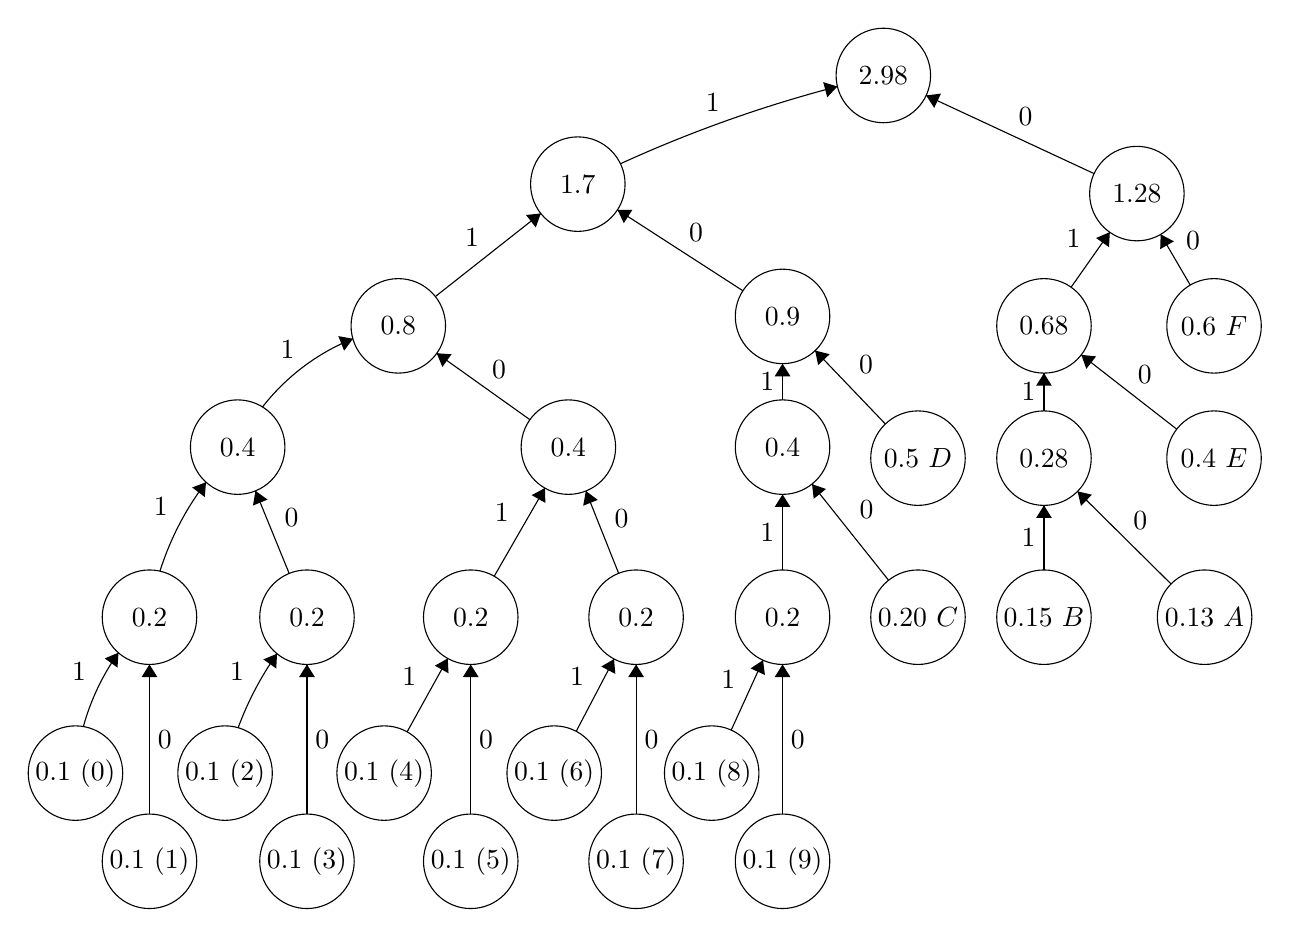
\begin{tikzpicture}[scale=0.2]
\tikzstyle{every node}+=[inner sep=0pt]
\draw [black] (3,-48.3) circle (3);
\draw (3,-48.3) node {$0.1\mbox{ }(0)$};
\draw [black] (7.7,-53.9) circle (3);
\draw (7.7,-53.9) node {$0.1\mbox{ }(1)$};
\draw [black] (12.5,-48.3) circle (3);
\draw (12.5,-48.3) node {$0.1\mbox{ }(2)$};
\draw [black] (74.7,-38.4) circle (3);
\draw (74.7,-38.4) node {$0.13\mbox{ }A$};
\draw [black] (56.5,-38.4) circle (3);
\draw (56.5,-38.4) node {$0.20\mbox{ }C$};
\draw [black] (43.4,-48.3) circle (3);
\draw (43.4,-48.3) node {$0.1\mbox{ }(8)$};
\draw [black] (64.5,-38.4) circle (3);
\draw (64.5,-38.4) node {$0.15\mbox{ }B$};
\draw [black] (33.4,-48.3) circle (3);
\draw (33.4,-48.3) node {$0.1\mbox{ }(6)$};
\draw [black] (28.1,-53.9) circle (3);
\draw (28.1,-53.9) node {$0.1\mbox{ }(5)$};
\draw [black] (22.6,-48.3) circle (3);
\draw (22.6,-48.3) node {$0.1\mbox{ }(4)$};
\draw [black] (17.7,-53.9) circle (3);
\draw (17.7,-53.9) node {$0.1\mbox{ }(3)$};
\draw [black] (47.9,-53.9) circle (3);
\draw (47.9,-53.9) node {$0.1\mbox{ }(9)$};
\draw [black] (38.6,-53.9) circle (3);
\draw (38.6,-53.9) node {$0.1\mbox{ }(7)$};
\draw [black] (56.5,-28.3) circle (3);
\draw (56.5,-28.3) node {$0.5\mbox{ }D$};
\draw [black] (75.3,-28.3) circle (3);
\draw (75.3,-28.3) node {$0.4\mbox{ }E$};
\draw [black] (75.3,-19.9) circle (3);
\draw (75.3,-19.9) node {$0.6\mbox{ }F$};
\draw [black] (7.7,-38.4) circle (3);
\draw (7.7,-38.4) node {$0.2$};
\draw [black] (17.7,-38.4) circle (3);
\draw (17.7,-38.4) node {$0.2$};
\draw [black] (28.1,-38.4) circle (3);
\draw (28.1,-38.4) node {$0.2$};
\draw [black] (38.6,-38.4) circle (3);
\draw (38.6,-38.4) node {$0.2$};
\draw [black] (47.9,-38.4) circle (3);
\draw (47.9,-38.4) node {$0.2$};
\draw [black] (64.5,-28.3) circle (3);
\draw (64.5,-28.3) node {$0.28$};
\draw [black] (13.3,-27.6) circle (3);
\draw (13.3,-27.6) node {$0.4$};
\draw [black] (64.5,-19.9) circle (3);
\draw (64.5,-19.9) node {$0.68$};
\draw [black] (34.3,-27.6) circle (3);
\draw (34.3,-27.6) node {$0.4$};
\draw [black] (47.9,-27.6) circle (3);
\draw (47.9,-27.6) node {$0.4$};
\draw [black] (23.5,-19.9) circle (3);
\draw (23.5,-19.9) node {$0.8$};
\draw [black] (47.9,-19.3) circle (3);
\draw (47.9,-19.3) node {$0.9$};
\draw [black] (70.4,-11.5) circle (3);
\draw (70.4,-11.5) node {$1.28$};
\draw [black] (34.9,-10.9) circle (3);
\draw (34.9,-10.9) node {$1.7$};
\draw [black] (54.3,-4) circle (3);
\draw (54.3,-4) node {$2.98$};
\draw [black] (3.501,-45.347) arc (164.61835:144.58982:14.936);
\fill [black] (5.73,-40.65) -- (4.86,-41.02) -- (5.67,-41.6);
\draw (3.7,-41.85) node [left] {$1$};
\draw [black] (7.7,-50.9) -- (7.7,-41.4);
\fill [black] (7.7,-41.4) -- (7.2,-42.2) -- (8.2,-42.2);
\draw (8.2,-46.15) node [right] {$0$};
\draw [black] (13.329,-45.42) arc (159.74699:144.83138:20.461);
\fill [black] (15.8,-40.72) -- (14.93,-41.08) -- (15.75,-41.66);
\draw (13.73,-41.84) node [left] {$1$};
\draw [black] (17.7,-50.9) -- (17.7,-41.4);
\fill [black] (17.7,-41.4) -- (17.2,-42.2) -- (18.2,-42.2);
\draw (18.2,-46.15) node [right] {$0$};
\draw [black] (24.06,-45.68) -- (26.64,-41.02);
\fill [black] (26.64,-41.02) -- (25.82,-41.48) -- (26.69,-41.96);
\draw (24.68,-42.15) node [left] {$1$};
\draw [black] (28.1,-50.9) -- (28.1,-41.4);
\fill [black] (28.1,-41.4) -- (27.6,-42.2) -- (28.6,-42.2);
\draw (28.6,-46.15) node [right] {$0$};
\draw [black] (34.8,-45.64) -- (37.2,-41.06);
\fill [black] (37.2,-41.06) -- (36.39,-41.53) -- (37.28,-42);
\draw (35.32,-42.2) node [left] {$1$};
\draw [black] (38.6,-50.9) -- (38.6,-41.4);
\fill [black] (38.6,-41.4) -- (38.1,-42.2) -- (39.1,-42.2);
\draw (39.1,-46.15) node [right] {$0$};
\draw [black] (44.64,-45.57) -- (46.66,-41.13);
\fill [black] (46.66,-41.13) -- (45.87,-41.65) -- (46.78,-42.07);
\draw (44.93,-42.34) node [left] {$1$};
\draw [black] (47.9,-50.9) -- (47.9,-41.4);
\fill [black] (47.9,-41.4) -- (47.4,-42.2) -- (48.4,-42.2);
\draw (48.4,-46.15) node [right] {$0$};
\draw [black] (72.57,-36.29) -- (66.63,-30.41);
\fill [black] (66.63,-30.41) -- (66.85,-31.33) -- (67.55,-30.62);
\draw (70.62,-32.87) node [above] {$0$};
\draw [black] (64.5,-35.4) -- (64.5,-31.3);
\fill [black] (64.5,-31.3) -- (64,-32.1) -- (65,-32.1);
\draw (64,-33.35) node [left] {$1$};
\draw [black] (8.365,-35.478) arc (162.52781:142.65704:18.447);
\fill [black] (11.29,-29.83) -- (10.41,-30.16) -- (11.21,-30.77);
\draw (8.9,-31.38) node [left] {$1$};
\draw [black] (29.59,-35.8) -- (32.81,-30.2);
\fill [black] (32.81,-30.2) -- (31.97,-30.65) -- (32.84,-31.14);
\draw (30.54,-31.77) node [left] {$1$};
\draw [black] (37.49,-35.61) -- (35.41,-30.39);
\fill [black] (35.41,-30.39) -- (35.24,-31.32) -- (36.17,-30.95);
\draw (37.2,-32.12) node [right] {$0$};
\draw [black] (47.9,-35.4) -- (47.9,-30.6);
\fill [black] (47.9,-30.6) -- (47.4,-31.4) -- (48.4,-31.4);
\draw (47.4,-33) node [left] {$1$};
\draw [black] (54.63,-36.05) -- (49.77,-29.95);
\fill [black] (49.77,-29.95) -- (49.88,-30.88) -- (50.66,-30.26);
\draw (52.76,-31.58) node [right] {$0$};
\draw [black] (16.57,-35.62) -- (14.43,-30.38);
\fill [black] (14.43,-30.38) -- (14.27,-31.31) -- (15.2,-30.93);
\draw (16.24,-32.1) node [right] {$0$};
\draw [black] (64.5,-25.3) -- (64.5,-22.9);
\fill [black] (64.5,-22.9) -- (64,-23.7) -- (65,-23.7);
\draw (64,-24.1) node [left] {$1$};
\draw [black] (72.93,-26.46) -- (66.87,-21.74);
\fill [black] (66.87,-21.74) -- (67.19,-22.63) -- (67.81,-21.84);
\draw (70.91,-23.6) node [above] {$0$};
\draw [black] (14.874,-25.053) arc (142.09198:112.00647:13.868);
\fill [black] (20.62,-20.72) -- (19.69,-20.55) -- (20.06,-21.48);
\draw (16.46,-22.01) node [above] {$1$};
\draw [black] (31.86,-25.86) -- (25.94,-21.64);
\fill [black] (25.94,-21.64) -- (26.3,-22.51) -- (26.88,-21.7);
\draw (29.9,-23.25) node [above] {$0$};
\draw [black] (47.9,-24.6) -- (47.9,-22.3);
\fill [black] (47.9,-22.3) -- (47.4,-23.1) -- (48.4,-23.1);
\draw (47.4,-23.45) node [left] {$1$};
\draw [black] (54.43,-26.13) -- (49.97,-21.47);
\fill [black] (49.97,-21.47) -- (50.16,-22.39) -- (50.89,-21.7);
\draw (52.73,-22.33) node [right] {$0$};
\draw [black] (25.85,-18.04) -- (32.55,-12.76);
\fill [black] (32.55,-12.76) -- (31.61,-12.86) -- (32.23,-13.65);
\draw (28.19,-14.9) node [above] {$1$};
\draw [black] (45.38,-17.67) -- (37.42,-12.53);
\fill [black] (37.42,-12.53) -- (37.82,-13.38) -- (38.36,-12.54);
\draw (42.4,-14.6) node [above] {$0$};
\draw [black] (66.22,-17.45) -- (68.68,-13.95);
\fill [black] (68.68,-13.95) -- (67.81,-14.32) -- (68.63,-14.9);
\draw (66.86,-14.34) node [left] {$1$};
\draw [black] (73.79,-17.31) -- (71.91,-14.09);
\fill [black] (71.91,-14.09) -- (71.88,-15.03) -- (72.75,-14.53);
\draw (73.5,-14.46) node [right] {$0$};
\draw [black] (37.606,-9.605) arc (114.56017:104.59773:84.21);
\fill [black] (51.38,-4.7) -- (50.48,-4.42) -- (50.74,-5.39);
\draw (43.47,-6.33) node [above] {$1$};
\draw [black] (67.68,-10.23) -- (57.02,-5.27);
\fill [black] (57.02,-5.27) -- (57.53,-6.06) -- (57.96,-5.15);
\draw (63.33,-7.24) node [above] {$0$};
\end{tikzpicture}
\end{center}

Daraus folgt entlang der Pfeile der Code:

\begin{description}
\item[0] 11111
\item[1] 11110
\item[2] 11101
\item[3] 11100
\item[4] 11011
\item[5] 11010
\item[6] 11001
\item[7] 11000
\item[8] 10111
\item[9] 10110
\item[A] 0110
\item[B] 0111
\item[C] 1010
\item[D] 100
\item[E] 010
\item[F] 00
\end{description}

Die Code-Länge ist 5 (entspricht der Tiefe des Baums).

\item Der Baum ist nicht eindeutig.

Alternative Darstellungen:

\begin{center}
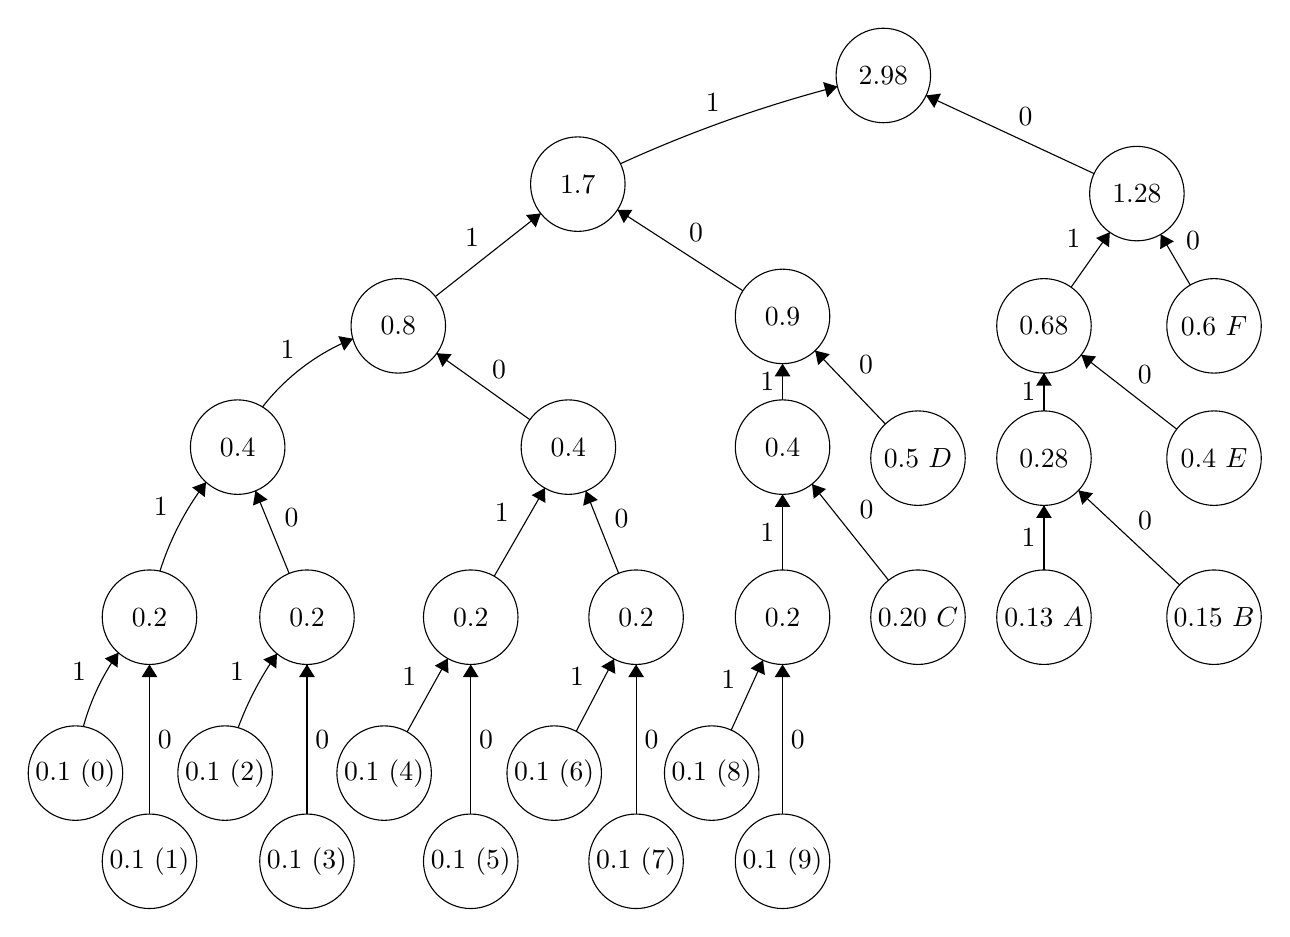
\begin{tikzpicture}[scale=0.2]
\tikzstyle{every node}+=[inner sep=0pt]
\draw [black] (3,-48.3) circle (3);
\draw (3,-48.3) node {$0.1\mbox{ }(0)$};
\draw [black] (7.7,-53.9) circle (3);
\draw (7.7,-53.9) node {$0.1\mbox{ }(1)$};
\draw [black] (12.5,-48.3) circle (3);
\draw (12.5,-48.3) node {$0.1\mbox{ }(2)$};
\draw [black] (64.5,-38.4) circle (3);
\draw (64.5,-38.4) node {$0.13\mbox{ }A$};
\draw [black] (56.5,-38.4) circle (3);
\draw (56.5,-38.4) node {$0.20\mbox{ }C$};
\draw [black] (43.4,-48.3) circle (3);
\draw (43.4,-48.3) node {$0.1\mbox{ }(8)$};
\draw [black] (75.3,-38.4) circle (3);
\draw (75.3,-38.4) node {$0.15\mbox{ }B$};
\draw [black] (33.4,-48.3) circle (3);
\draw (33.4,-48.3) node {$0.1\mbox{ }(6)$};
\draw [black] (28.1,-53.9) circle (3);
\draw (28.1,-53.9) node {$0.1\mbox{ }(5)$};
\draw [black] (22.6,-48.3) circle (3);
\draw (22.6,-48.3) node {$0.1\mbox{ }(4)$};
\draw [black] (17.7,-53.9) circle (3);
\draw (17.7,-53.9) node {$0.1\mbox{ }(3)$};
\draw [black] (47.9,-53.9) circle (3);
\draw (47.9,-53.9) node {$0.1\mbox{ }(9)$};
\draw [black] (38.6,-53.9) circle (3);
\draw (38.6,-53.9) node {$0.1\mbox{ }(7)$};
\draw [black] (56.5,-28.3) circle (3);
\draw (56.5,-28.3) node {$0.5\mbox{ }D$};
\draw [black] (75.3,-28.3) circle (3);
\draw (75.3,-28.3) node {$0.4\mbox{ }E$};
\draw [black] (75.3,-19.9) circle (3);
\draw (75.3,-19.9) node {$0.6\mbox{ }F$};
\draw [black] (7.7,-38.4) circle (3);
\draw (7.7,-38.4) node {$0.2$};
\draw [black] (17.7,-38.4) circle (3);
\draw (17.7,-38.4) node {$0.2$};
\draw [black] (28.1,-38.4) circle (3);
\draw (28.1,-38.4) node {$0.2$};
\draw [black] (38.6,-38.4) circle (3);
\draw (38.6,-38.4) node {$0.2$};
\draw [black] (47.9,-38.4) circle (3);
\draw (47.9,-38.4) node {$0.2$};
\draw [black] (64.5,-28.3) circle (3);
\draw (64.5,-28.3) node {$0.28$};
\draw [black] (13.3,-27.6) circle (3);
\draw (13.3,-27.6) node {$0.4$};
\draw [black] (64.5,-19.9) circle (3);
\draw (64.5,-19.9) node {$0.68$};
\draw [black] (34.3,-27.6) circle (3);
\draw (34.3,-27.6) node {$0.4$};
\draw [black] (47.9,-27.6) circle (3);
\draw (47.9,-27.6) node {$0.4$};
\draw [black] (23.5,-19.9) circle (3);
\draw (23.5,-19.9) node {$0.8$};
\draw [black] (47.9,-19.3) circle (3);
\draw (47.9,-19.3) node {$0.9$};
\draw [black] (70.4,-11.5) circle (3);
\draw (70.4,-11.5) node {$1.28$};
\draw [black] (34.9,-10.9) circle (3);
\draw (34.9,-10.9) node {$1.7$};
\draw [black] (54.3,-4) circle (3);
\draw (54.3,-4) node {$2.98$};
\draw [black] (3.501,-45.347) arc (164.61835:144.58982:14.936);
\fill [black] (5.73,-40.65) -- (4.86,-41.02) -- (5.67,-41.6);
\draw (3.7,-41.85) node [left] {$1$};
\draw [black] (7.7,-50.9) -- (7.7,-41.4);
\fill [black] (7.7,-41.4) -- (7.2,-42.2) -- (8.2,-42.2);
\draw (8.2,-46.15) node [right] {$0$};
\draw [black] (13.329,-45.42) arc (159.74699:144.83138:20.461);
\fill [black] (15.8,-40.72) -- (14.93,-41.08) -- (15.75,-41.66);
\draw (13.73,-41.84) node [left] {$1$};
\draw [black] (17.7,-50.9) -- (17.7,-41.4);
\fill [black] (17.7,-41.4) -- (17.2,-42.2) -- (18.2,-42.2);
\draw (18.2,-46.15) node [right] {$0$};
\draw [black] (24.06,-45.68) -- (26.64,-41.02);
\fill [black] (26.64,-41.02) -- (25.82,-41.48) -- (26.69,-41.96);
\draw (24.68,-42.15) node [left] {$1$};
\draw [black] (28.1,-50.9) -- (28.1,-41.4);
\fill [black] (28.1,-41.4) -- (27.6,-42.2) -- (28.6,-42.2);
\draw (28.6,-46.15) node [right] {$0$};
\draw [black] (34.8,-45.64) -- (37.2,-41.06);
\fill [black] (37.2,-41.06) -- (36.39,-41.53) -- (37.28,-42);
\draw (35.32,-42.2) node [left] {$1$};
\draw [black] (38.6,-50.9) -- (38.6,-41.4);
\fill [black] (38.6,-41.4) -- (38.1,-42.2) -- (39.1,-42.2);
\draw (39.1,-46.15) node [right] {$0$};
\draw [black] (44.64,-45.57) -- (46.66,-41.13);
\fill [black] (46.66,-41.13) -- (45.87,-41.65) -- (46.78,-42.07);
\draw (44.93,-42.34) node [left] {$1$};
\draw [black] (47.9,-50.9) -- (47.9,-41.4);
\fill [black] (47.9,-41.4) -- (47.4,-42.2) -- (48.4,-42.2);
\draw (48.4,-46.15) node [right] {$0$};
\draw [black] (64.5,-35.4) -- (64.5,-31.3);
\fill [black] (64.5,-31.3) -- (64,-32.1) -- (65,-32.1);
\draw (64,-33.35) node [left] {$1$};
\draw [black] (73.11,-36.35) -- (66.69,-30.35);
\fill [black] (66.69,-30.35) -- (66.93,-31.26) -- (67.62,-30.53);
\draw (70.92,-32.87) node [above] {$0$};
\draw [black] (8.365,-35.478) arc (162.52781:142.65704:18.447);
\fill [black] (11.29,-29.83) -- (10.41,-30.16) -- (11.21,-30.77);
\draw (8.9,-31.38) node [left] {$1$};
\draw [black] (29.59,-35.8) -- (32.81,-30.2);
\fill [black] (32.81,-30.2) -- (31.97,-30.65) -- (32.84,-31.14);
\draw (30.54,-31.77) node [left] {$1$};
\draw [black] (37.49,-35.61) -- (35.41,-30.39);
\fill [black] (35.41,-30.39) -- (35.24,-31.32) -- (36.17,-30.95);
\draw (37.2,-32.12) node [right] {$0$};
\draw [black] (47.9,-35.4) -- (47.9,-30.6);
\fill [black] (47.9,-30.6) -- (47.4,-31.4) -- (48.4,-31.4);
\draw (47.4,-33) node [left] {$1$};
\draw [black] (54.63,-36.05) -- (49.77,-29.95);
\fill [black] (49.77,-29.95) -- (49.88,-30.88) -- (50.66,-30.26);
\draw (52.76,-31.58) node [right] {$0$};
\draw [black] (16.57,-35.62) -- (14.43,-30.38);
\fill [black] (14.43,-30.38) -- (14.27,-31.31) -- (15.2,-30.93);
\draw (16.24,-32.1) node [right] {$0$};
\draw [black] (64.5,-25.3) -- (64.5,-22.9);
\fill [black] (64.5,-22.9) -- (64,-23.7) -- (65,-23.7);
\draw (64,-24.1) node [left] {$1$};
\draw [black] (72.93,-26.46) -- (66.87,-21.74);
\fill [black] (66.87,-21.74) -- (67.19,-22.63) -- (67.81,-21.84);
\draw (70.91,-23.6) node [above] {$0$};
\draw [black] (14.874,-25.053) arc (142.09198:112.00647:13.868);
\fill [black] (20.62,-20.72) -- (19.69,-20.55) -- (20.06,-21.48);
\draw (16.46,-22.01) node [above] {$1$};
\draw [black] (31.86,-25.86) -- (25.94,-21.64);
\fill [black] (25.94,-21.64) -- (26.3,-22.51) -- (26.88,-21.7);
\draw (29.9,-23.25) node [above] {$0$};
\draw [black] (47.9,-24.6) -- (47.9,-22.3);
\fill [black] (47.9,-22.3) -- (47.4,-23.1) -- (48.4,-23.1);
\draw (47.4,-23.45) node [left] {$1$};
\draw [black] (54.43,-26.13) -- (49.97,-21.47);
\fill [black] (49.97,-21.47) -- (50.16,-22.39) -- (50.89,-21.7);
\draw (52.73,-22.33) node [right] {$0$};
\draw [black] (25.85,-18.04) -- (32.55,-12.76);
\fill [black] (32.55,-12.76) -- (31.61,-12.86) -- (32.23,-13.65);
\draw (28.19,-14.9) node [above] {$1$};
\draw [black] (45.38,-17.67) -- (37.42,-12.53);
\fill [black] (37.42,-12.53) -- (37.82,-13.38) -- (38.36,-12.54);
\draw (42.4,-14.6) node [above] {$0$};
\draw [black] (66.22,-17.45) -- (68.68,-13.95);
\fill [black] (68.68,-13.95) -- (67.81,-14.32) -- (68.63,-14.9);
\draw (66.86,-14.34) node [left] {$1$};
\draw [black] (73.79,-17.31) -- (71.91,-14.09);
\fill [black] (71.91,-14.09) -- (71.88,-15.03) -- (72.75,-14.53);
\draw (73.5,-14.46) node [right] {$0$};
\draw [black] (37.606,-9.605) arc (114.56017:104.59773:84.21);
\fill [black] (51.38,-4.7) -- (50.48,-4.42) -- (50.74,-5.39);
\draw (43.47,-6.33) node [above] {$1$};
\draw [black] (67.68,-10.23) -- (57.02,-5.27);
\fill [black] (57.02,-5.27) -- (57.53,-6.06) -- (57.96,-5.15);
\draw (63.33,-7.24) node [above] {$0$};
\end{tikzpicture}
\end{center}
(A und B vertauscht)

\begin{center}
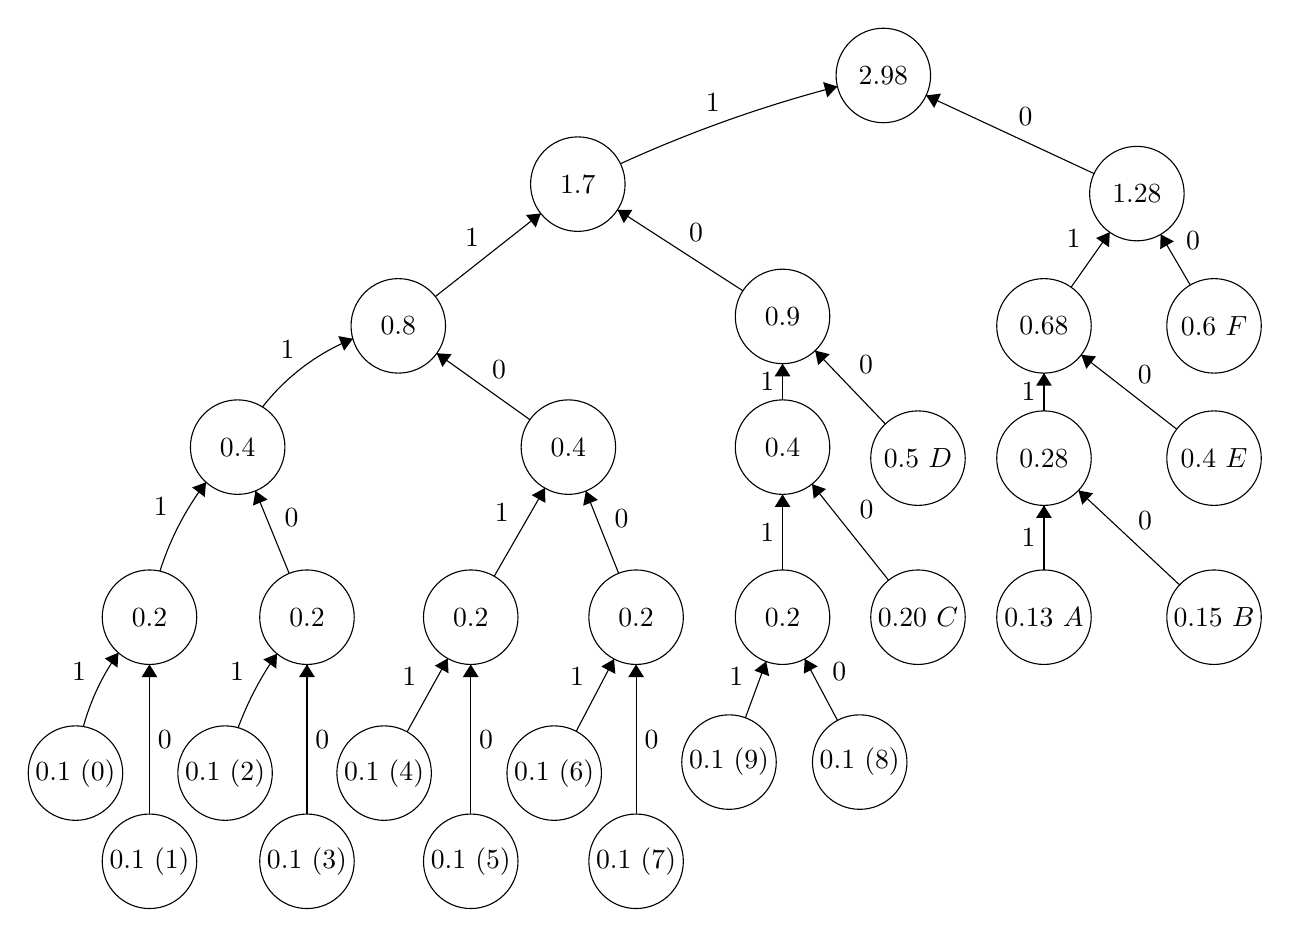
\begin{tikzpicture}[scale=0.2]
\tikzstyle{every node}+=[inner sep=0pt]
\draw [black] (3,-48.3) circle (3);
\draw (3,-48.3) node {$0.1\mbox{ }(0)$};
\draw [black] (7.7,-53.9) circle (3);
\draw (7.7,-53.9) node {$0.1\mbox{ }(1)$};
\draw [black] (12.5,-48.3) circle (3);
\draw (12.5,-48.3) node {$0.1\mbox{ }(2)$};
\draw [black] (64.5,-38.4) circle (3);
\draw (64.5,-38.4) node {$0.13\mbox{ }A$};
\draw [black] (56.5,-38.4) circle (3);
\draw (56.5,-38.4) node {$0.20\mbox{ }C$};
\draw [black] (52.8,-47.6) circle (3);
\draw (52.8,-47.6) node {$0.1\mbox{ }(8)$};
\draw [black] (75.3,-38.4) circle (3);
\draw (75.3,-38.4) node {$0.15\mbox{ }B$};
\draw [black] (33.4,-48.3) circle (3);
\draw (33.4,-48.3) node {$0.1\mbox{ }(6)$};
\draw [black] (28.1,-53.9) circle (3);
\draw (28.1,-53.9) node {$0.1\mbox{ }(5)$};
\draw [black] (22.6,-48.3) circle (3);
\draw (22.6,-48.3) node {$0.1\mbox{ }(4)$};
\draw [black] (17.7,-53.9) circle (3);
\draw (17.7,-53.9) node {$0.1\mbox{ }(3)$};
\draw [black] (44.5,-47.6) circle (3);
\draw (44.5,-47.6) node {$0.1\mbox{ }(9)$};
\draw [black] (38.6,-53.9) circle (3);
\draw (38.6,-53.9) node {$0.1\mbox{ }(7)$};
\draw [black] (56.5,-28.3) circle (3);
\draw (56.5,-28.3) node {$0.5\mbox{ }D$};
\draw [black] (75.3,-28.3) circle (3);
\draw (75.3,-28.3) node {$0.4\mbox{ }E$};
\draw [black] (75.3,-19.9) circle (3);
\draw (75.3,-19.9) node {$0.6\mbox{ }F$};
\draw [black] (7.7,-38.4) circle (3);
\draw (7.7,-38.4) node {$0.2$};
\draw [black] (17.7,-38.4) circle (3);
\draw (17.7,-38.4) node {$0.2$};
\draw [black] (28.1,-38.4) circle (3);
\draw (28.1,-38.4) node {$0.2$};
\draw [black] (38.6,-38.4) circle (3);
\draw (38.6,-38.4) node {$0.2$};
\draw [black] (47.9,-38.4) circle (3);
\draw (47.9,-38.4) node {$0.2$};
\draw [black] (64.5,-28.3) circle (3);
\draw (64.5,-28.3) node {$0.28$};
\draw [black] (13.3,-27.6) circle (3);
\draw (13.3,-27.6) node {$0.4$};
\draw [black] (64.5,-19.9) circle (3);
\draw (64.5,-19.9) node {$0.68$};
\draw [black] (34.3,-27.6) circle (3);
\draw (34.3,-27.6) node {$0.4$};
\draw [black] (47.9,-27.6) circle (3);
\draw (47.9,-27.6) node {$0.4$};
\draw [black] (23.5,-19.9) circle (3);
\draw (23.5,-19.9) node {$0.8$};
\draw [black] (47.9,-19.3) circle (3);
\draw (47.9,-19.3) node {$0.9$};
\draw [black] (70.4,-11.5) circle (3);
\draw (70.4,-11.5) node {$1.28$};
\draw [black] (34.9,-10.9) circle (3);
\draw (34.9,-10.9) node {$1.7$};
\draw [black] (54.3,-4) circle (3);
\draw (54.3,-4) node {$2.98$};
\draw [black] (3.501,-45.347) arc (164.61835:144.58982:14.936);
\fill [black] (5.73,-40.65) -- (4.86,-41.02) -- (5.67,-41.6);
\draw (3.7,-41.85) node [left] {$1$};
\draw [black] (7.7,-50.9) -- (7.7,-41.4);
\fill [black] (7.7,-41.4) -- (7.2,-42.2) -- (8.2,-42.2);
\draw (8.2,-46.15) node [right] {$0$};
\draw [black] (13.329,-45.42) arc (159.74699:144.83138:20.461);
\fill [black] (15.8,-40.72) -- (14.93,-41.08) -- (15.75,-41.66);
\draw (13.73,-41.84) node [left] {$1$};
\draw [black] (17.7,-50.9) -- (17.7,-41.4);
\fill [black] (17.7,-41.4) -- (17.2,-42.2) -- (18.2,-42.2);
\draw (18.2,-46.15) node [right] {$0$};
\draw [black] (24.06,-45.68) -- (26.64,-41.02);
\fill [black] (26.64,-41.02) -- (25.82,-41.48) -- (26.69,-41.96);
\draw (24.68,-42.15) node [left] {$1$};
\draw [black] (28.1,-50.9) -- (28.1,-41.4);
\fill [black] (28.1,-41.4) -- (27.6,-42.2) -- (28.6,-42.2);
\draw (28.6,-46.15) node [right] {$0$};
\draw [black] (34.8,-45.64) -- (37.2,-41.06);
\fill [black] (37.2,-41.06) -- (36.39,-41.53) -- (37.28,-42);
\draw (35.32,-42.2) node [left] {$1$};
\draw [black] (38.6,-50.9) -- (38.6,-41.4);
\fill [black] (38.6,-41.4) -- (38.1,-42.2) -- (39.1,-42.2);
\draw (39.1,-46.15) node [right] {$0$};
\draw [black] (51.39,-44.95) -- (49.31,-41.05);
\fill [black] (49.31,-41.05) -- (49.25,-41.99) -- (50.13,-41.52);
\draw (51.03,-41.84) node [right] {$0$};
\draw [black] (45.54,-44.79) -- (46.86,-41.21);
\fill [black] (46.86,-41.21) -- (46.11,-41.79) -- (47.05,-42.14);
\draw (45.44,-42.2) node [left] {$1$};
\draw [black] (64.5,-35.4) -- (64.5,-31.3);
\fill [black] (64.5,-31.3) -- (64,-32.1) -- (65,-32.1);
\draw (64,-33.35) node [left] {$1$};
\draw [black] (73.11,-36.35) -- (66.69,-30.35);
\fill [black] (66.69,-30.35) -- (66.93,-31.26) -- (67.62,-30.53);
\draw (70.92,-32.87) node [above] {$0$};
\draw [black] (8.365,-35.478) arc (162.52781:142.65704:18.447);
\fill [black] (11.29,-29.83) -- (10.41,-30.16) -- (11.21,-30.77);
\draw (8.9,-31.38) node [left] {$1$};
\draw [black] (29.59,-35.8) -- (32.81,-30.2);
\fill [black] (32.81,-30.2) -- (31.97,-30.65) -- (32.84,-31.14);
\draw (30.54,-31.77) node [left] {$1$};
\draw [black] (37.49,-35.61) -- (35.41,-30.39);
\fill [black] (35.41,-30.39) -- (35.24,-31.32) -- (36.17,-30.95);
\draw (37.2,-32.12) node [right] {$0$};
\draw [black] (47.9,-35.4) -- (47.9,-30.6);
\fill [black] (47.9,-30.6) -- (47.4,-31.4) -- (48.4,-31.4);
\draw (47.4,-33) node [left] {$1$};
\draw [black] (54.63,-36.05) -- (49.77,-29.95);
\fill [black] (49.77,-29.95) -- (49.88,-30.88) -- (50.66,-30.26);
\draw (52.76,-31.58) node [right] {$0$};
\draw [black] (16.57,-35.62) -- (14.43,-30.38);
\fill [black] (14.43,-30.38) -- (14.27,-31.31) -- (15.2,-30.93);
\draw (16.24,-32.1) node [right] {$0$};
\draw [black] (64.5,-25.3) -- (64.5,-22.9);
\fill [black] (64.5,-22.9) -- (64,-23.7) -- (65,-23.7);
\draw (64,-24.1) node [left] {$1$};
\draw [black] (72.93,-26.46) -- (66.87,-21.74);
\fill [black] (66.87,-21.74) -- (67.19,-22.63) -- (67.81,-21.84);
\draw (70.91,-23.6) node [above] {$0$};
\draw [black] (14.874,-25.053) arc (142.09198:112.00647:13.868);
\fill [black] (20.62,-20.72) -- (19.69,-20.55) -- (20.06,-21.48);
\draw (16.46,-22.01) node [above] {$1$};
\draw [black] (31.86,-25.86) -- (25.94,-21.64);
\fill [black] (25.94,-21.64) -- (26.3,-22.51) -- (26.88,-21.7);
\draw (29.9,-23.25) node [above] {$0$};
\draw [black] (47.9,-24.6) -- (47.9,-22.3);
\fill [black] (47.9,-22.3) -- (47.4,-23.1) -- (48.4,-23.1);
\draw (47.4,-23.45) node [left] {$1$};
\draw [black] (54.43,-26.13) -- (49.97,-21.47);
\fill [black] (49.97,-21.47) -- (50.16,-22.39) -- (50.89,-21.7);
\draw (52.73,-22.33) node [right] {$0$};
\draw [black] (25.85,-18.04) -- (32.55,-12.76);
\fill [black] (32.55,-12.76) -- (31.61,-12.86) -- (32.23,-13.65);
\draw (28.19,-14.9) node [above] {$1$};
\draw [black] (45.38,-17.67) -- (37.42,-12.53);
\fill [black] (37.42,-12.53) -- (37.82,-13.38) -- (38.36,-12.54);
\draw (42.4,-14.6) node [above] {$0$};
\draw [black] (66.22,-17.45) -- (68.68,-13.95);
\fill [black] (68.68,-13.95) -- (67.81,-14.32) -- (68.63,-14.9);
\draw (66.86,-14.34) node [left] {$1$};
\draw [black] (73.79,-17.31) -- (71.91,-14.09);
\fill [black] (71.91,-14.09) -- (71.88,-15.03) -- (72.75,-14.53);
\draw (73.5,-14.46) node [right] {$0$};
\draw [black] (37.606,-9.605) arc (114.56017:104.59773:84.21);
\fill [black] (51.38,-4.7) -- (50.48,-4.42) -- (50.74,-5.39);
\draw (43.47,-6.33) node [above] {$1$};
\draw [black] (67.68,-10.23) -- (57.02,-5.27);
\fill [black] (57.02,-5.27) -- (57.53,-6.06) -- (57.96,-5.15);
\draw (63.33,-7.24) node [above] {$0$};
\end{tikzpicture}
\end{center}
(8 und 9 vertauscht)

\item Indem kein Binär-, sondern ein regulärer Baum mit beispielsweise 3 Kindkoten pro Knoten verwendet wird.

\item Regulärer 3-kindknotiger Baum:

\begin{center}
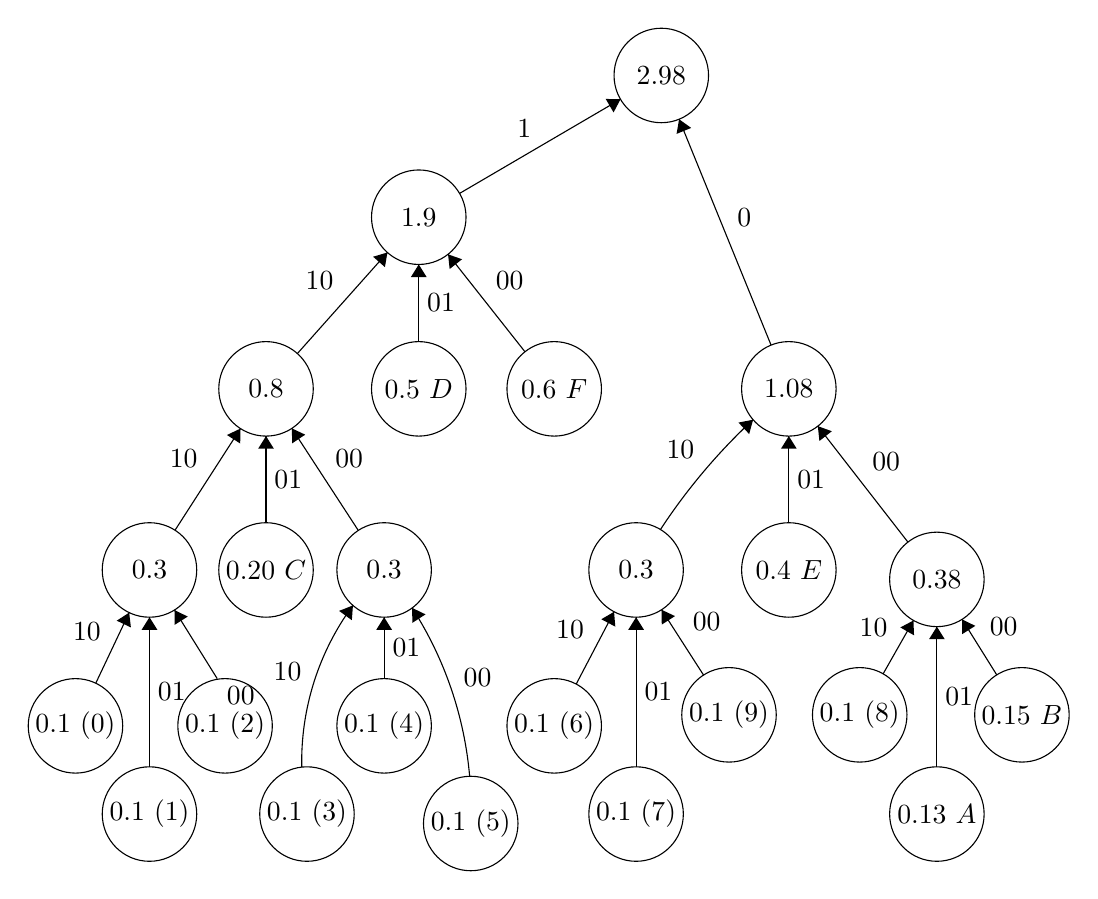
\begin{tikzpicture}[scale=0.2]
\tikzstyle{every node}+=[inner sep=0pt]
\draw [black] (3,-48.3) circle (3);
\draw (3,-48.3) node {$0.1\mbox{ }(0)$};
\draw [black] (7.7,-53.9) circle (3);
\draw (7.7,-53.9) node {$0.1\mbox{ }(1)$};
\draw [black] (12.5,-48.3) circle (3);
\draw (12.5,-48.3) node {$0.1\mbox{ }(2)$};
\draw [black] (57.7,-53.9) circle (3);
\draw (57.7,-53.9) node {$0.13\mbox{ }A$};
\draw [black] (15.1,-38.4) circle (3);
\draw (15.1,-38.4) node {$0.20\mbox{ }C$};
\draw [black] (52.8,-47.6) circle (3);
\draw (52.8,-47.6) node {$0.1\mbox{ }(8)$};
\draw [black] (63.1,-47.6) circle (3);
\draw (63.1,-47.6) node {$0.15\mbox{ }B$};
\draw [black] (33.4,-48.3) circle (3);
\draw (33.4,-48.3) node {$0.1\mbox{ }(6)$};
\draw [black] (28.1,-54.5) circle (3);
\draw (28.1,-54.5) node {$0.1\mbox{ }(5)$};
\draw [black] (22.6,-48.3) circle (3);
\draw (22.6,-48.3) node {$0.1\mbox{ }(4)$};
\draw [black] (17.7,-53.9) circle (3);
\draw (17.7,-53.9) node {$0.1\mbox{ }(3)$};
\draw [black] (44.5,-47.6) circle (3);
\draw (44.5,-47.6) node {$0.1\mbox{ }(9)$};
\draw [black] (38.6,-53.9) circle (3);
\draw (38.6,-53.9) node {$0.1\mbox{ }(7)$};
\draw [black] (24.8,-26.9) circle (3);
\draw (24.8,-26.9) node {$0.5\mbox{ }D$};
\draw [black] (48.3,-38.4) circle (3);
\draw (48.3,-38.4) node {$0.4\mbox{ }E$};
\draw [black] (33.4,-26.9) circle (3);
\draw (33.4,-26.9) node {$0.6\mbox{ }F$};
\draw [black] (7.7,-38.4) circle (3);
\draw (7.7,-38.4) node {$0.3$};
\draw [black] (22.6,-38.4) circle (3);
\draw (22.6,-38.4) node {$0.3$};
\draw [black] (38.6,-38.4) circle (3);
\draw (38.6,-38.4) node {$0.3$};
\draw [black] (57.7,-39) circle (3);
\draw (57.7,-39) node {$0.38$};
\draw [black] (15.1,-26.9) circle (3);
\draw (15.1,-26.9) node {$0.8$};
\draw [black] (48.3,-26.9) circle (3);
\draw (48.3,-26.9) node {$1.08$};
\draw [black] (24.8,-16) circle (3);
\draw (24.8,-16) node {$1.9$};
\draw [black] (40.2,-7) circle (3);
\draw (40.2,-7) node {$2.98$};
\draw [black] (4.29,-45.59) -- (6.41,-41.11);
\fill [black] (6.41,-41.11) -- (5.62,-41.62) -- (6.52,-42.05);
\draw (4.64,-42.29) node [left] {$10$};
\draw [black] (7.7,-50.9) -- (7.7,-41.4);
\fill [black] (7.7,-41.4) -- (7.2,-42.2) -- (8.2,-42.2);
\draw (8.2,-46.15) node [right] {$01$};
\draw [black] (12,-45.3) -- (9.29,-40.95);
\draw (13.5,-45.8) node [below] {$00$};
\fill [black] (9.29,-40.95) -- (9.29,-41.89) -- (10.13,-41.36);
\draw [black] (17.369,-50.922) arc (-178.78974:-216.29678:16.761);
\fill [black] (20.62,-40.65) -- (19.74,-41) -- (20.55,-41.59);
\draw (17.38,-44.86) node [left] {$10$};
\draw [black] (22.6,-45.3) -- (22.6,-41.4);
\fill [black] (22.6,-41.4) -- (22.1,-42.2) -- (23.1,-42.2);
\draw (23.1,-43.35) node [right] {$01$};
\draw [black] (24.379,-40.813) arc (32.75319:4.96868:23.525);
\fill [black] (24.38,-40.81) -- (24.39,-41.76) -- (25.23,-41.22);
\draw (27.62,-45.21) node [right] {$00$};
\draw [black] (34.8,-45.64) -- (37.2,-41.06);
\fill [black] (37.2,-41.06) -- (36.39,-41.53) -- (37.28,-42);
\draw (35.32,-42.2) node [left] {$10$};
\draw [black] (38.6,-50.9) -- (38.6,-41.4);
\fill [black] (38.6,-41.4) -- (38.1,-42.2) -- (39.1,-42.2);
\draw (39.1,-46.15) node [right] {$01$};
\draw [black] (42.88,-45.07) -- (40.22,-40.93);
\fill [black] (40.22,-40.93) -- (40.23,-41.87) -- (41.07,-41.33);
\draw (42.17,-41.69) node [right] {$00$};
\draw [black] (54.29,-44.99) -- (56.21,-41.61);
\fill [black] (56.21,-41.61) -- (55.38,-42.05) -- (56.25,-42.55);
\draw (54.59,-42.08) node [left] {$10$};
\draw [black] (57.7,-50.9) -- (57.7,-42);
\fill [black] (57.7,-42) -- (57.2,-42.8) -- (58.2,-42.8);
\draw (58.2,-46.45) node [right] {$01$};
\draw [black] (61.5,-45.06) -- (59.3,-41.54);
\fill [black] (59.3,-41.54) -- (59.3,-42.48) -- (60.14,-41.95);
\draw (61.03,-42) node [right] {$00$};
\draw [black] (9.32,-35.88) -- (13.48,-29.42);
\fill [black] (13.48,-29.42) -- (12.62,-29.83) -- (13.46,-30.37);
\draw (10.78,-31.34) node [left] {$10$};
\draw [black] (15.1,-35.4) -- (15.1,-29.9);
\fill [black] (15.1,-29.9) -- (14.6,-30.7) -- (15.6,-30.7);
\draw (15.6,-32.65) node [right] {$01$};
\draw [black] (20.96,-35.89) -- (16.74,-29.41);
\fill [black] (16.74,-29.41) -- (16.76,-30.36) -- (17.59,-29.81);
\draw (19.47,-31.33) node [right] {$00$};
\draw [black] (40.146,-35.83) arc (146.71895:132.98725:38.153);
\fill [black] (46.03,-28.86) -- (45.1,-29.04) -- (45.78,-29.77);
\draw (42.33,-30.73) node [left] {$10$};
\draw [black] (48.3,-35.4) -- (48.3,-29.9);
\fill [black] (48.3,-29.9) -- (47.8,-30.7) -- (48.8,-30.7);
\draw (48.8,-32.65) node [right] {$01$};
\draw [black] (55.86,-36.63) -- (50.14,-29.27);
\fill [black] (50.14,-29.27) -- (50.24,-30.21) -- (51.03,-29.59);
\draw (53.57,-31.54) node [right] {$00$};
\draw [black] (17.09,-24.66) -- (22.81,-18.24);
\fill [black] (22.81,-18.24) -- (21.9,-18.51) -- (22.65,-19.17);
\draw (19.41,-20) node [left] {$10$};
\draw [black] (24.8,-23.9) -- (24.8,-19);
\fill [black] (24.8,-19) -- (24.3,-19.8) -- (25.3,-19.8);
\draw (25.3,-21.45) node [right] {$01$};
\draw [black] (31.54,-24.54) -- (26.66,-18.36);
\fill [black] (26.66,-18.36) -- (26.76,-19.29) -- (27.55,-18.67);
\draw (29.66,-20.03) node [right] {$00$};
\draw [black] (27.39,-14.49) -- (37.61,-8.51);
\fill [black] (37.61,-8.51) -- (36.67,-8.49) -- (37.17,-9.35);
\draw (31.5,-11) node [above] {$1$};
\draw [black] (47.17,-24.12) -- (41.33,-9.78);
\fill [black] (41.33,-9.78) -- (41.17,-10.71) -- (42.1,-10.33);
\draw (44.99,-16.05) node [right] {$0$};
\end{tikzpicture}
\end{center}

\item Nein, weil auch die einzelnen Zeichen von Binärdaten wiederkehrende Häufigkeiten aufweisen (0 wird beispielsweise relativ häufig auftauchen).

\end{enumerate}

\section*{Aufgabe 2}

\begin{enumerate}[1.]
\item Man kann Redundanz in die übertragenen Daten einbauen und dann die überschüssige Information verwenden, um Fehlererkennung bzw. -korrektur zu betreiben.

\item Die Kompression sollte vor der Chiffrierung erfolgen, weil das Ziel der Chiffrierung eine möglichst zufällige Verteilung der Zeichen ist. Dies hat negative Auswirkungen auf die Kompression, weil diese sich normalerweise wiederauftretende Muster bzw. ungleiche Auftretenswahrscheinlichkeiten zu Nutze macht. Die Fehlerkorrektur kommt sinnvollerweise erst am Ende, damit während dem Empfangen gleich als erstes die Fehleranalyse gemacht werden kann und nicht erst die Daten dechiffriert und dekomprimiert werden müssen.

Also: Kompression $\Rightarrow$ Chiffrierung $\Rightarrow$ Fehlerkorrektur beim Senden, Fehlerkorrektur $\Rightarrow$ Dechiffrierung $\Rightarrow$ Dekompression beim Empfangen.

\item

\begin{itemize}

\item Generatormatrix:
\begin{eqnarray*}
G = \begin{bmatrix}
1 & 1 & 1 & 0 & 0 & 0 & 0 \\
1 & 0 & 0 & 1 & 1 & 0 & 0 \\
0 & 1 & 0 & 1 & 0 & 1 & 0 \\
1 & 1 & 0 & 1 & 0 & 0 & 1 \\
\end{bmatrix}
\end{eqnarray*}

\item Allgemein:
\[
\begin{bmatrix} p_1 & p_2 & d_3 & p_4 & d_5 & d_6 & d_7 \end{bmatrix} = \begin{bmatrix} d_3 & d_5 & d_6 & d_7 \end{bmatrix} G
\]
Mögliche Codewörter:

\begin{tabular}{r||l|l|l||l}
$d_3d_5d_6d_7$ & $p_1 = d_3+d_5+d_7$ & $p_2=d_3+d_6+d_7$ & $p_4=d_5+d_6+d_7$ & $p_1p_2d_3p_4d_5d_6d_7$ \\\hline
0000 & 0 & 0 & 0 & 0000000 \\
0001 & 1 & 1 & 1 & 1101001 \\
0010 & 0 & 1 & 1 & 0101010 \\
0011 & 1 & 2=0 &2=0 & 1000011 \\
0100 & 1 & 0 &1 & 1001100 \\
0101 & 2=0 & 1 &2=0 & 0100101 \\
0110 & 1 & 1 &2=0 & 1100110 \\
0111 & 2=0 & 2=0  &3=1 & 0001111 \\
1000 & 1 & 1 &0 & 1110000 \\
1001 & 2=0 & 2=0 &1 & 0011001 \\
1010 & 1 & 2=0 &1 & 1011010 \\
1011 & 2=0 &3=1 &2=0 &0110011 \\
1100 & 2=0 &1 &1 & 0111100 \\
1101 & 3=1 &2=0 &2=0 & 1010101 \\
1110 & 2=0 &2=0 &2=0 & 0010110 \\
1111 & 3=1 &3=1 &3=1 & 1111111 \\
\end{tabular}

\item Indem wir die übertragenen Codewörter mit der Checkmatrix $H$ multiplizieren und 0 als Resultat erwarten.

\[
H = \begin{bmatrix}
0 & 0 & 0 & 1 & 1 & 1 & 1 \\
0 & 1 & 1 & 0 & 0 & 1 & 1 \\
1 & 0 & 1 & 0 & 1 & 0 & 1 \\
\end{bmatrix}
\]

Beispielsweise für das Datenwort 0010:
\[
H \begin{bmatrix}
0 & 1 & 0 & 1 & 0 & 1 & 0
\end{bmatrix}^T = \begin{bmatrix} 2 \\ 2 \\ 0 \end{bmatrix} = \begin{bmatrix} 0 \\ 0 \\ 0\end{bmatrix}
\]

Wenn hingegen ein Übertragungsfehler stattfindet, beispielsweise das dritte Bit gedreht ist:
\[
H \begin{bmatrix}
0 & 1 & 1 & 1 & 0 & 1 & 0
\end{bmatrix}^T = \begin{bmatrix} 2 \\ 3 \\ 1 \end{bmatrix} = \begin{bmatrix} 0 \\ 1 \\ 1\end{bmatrix}
\]

\item Der resultierende Vektor ist die binäre Repräsentation der Fehlerstelle: $011_b = 3$. Dementsprechend können wir diese Stelle korrigieren und erhalten das gültige, beabsichtigte Codewort.

\end{itemize}
\end{enumerate}

\end{document}
